% This part is to be filled by Johann
\subsection{1-tree lower bound}

\begin{frame}[t]{How To Get A 1-tree Lower Bound?}
  Start with an MST over $n-1$ edges (here vertex $4$ is left out):

  \begin{tikzpicture}
    \graph { subgraph K_n [n=5, clockwise, edges=gray];
      (1) --[thick] (2);
      (1) --[thick] (5);
      (1) --[thick] (3); };
    
  \end{tikzpicture}

  Then add the remaining vertex, and the two edges with lowest cost adjacent to that vertex:

  \begin{tikzpicture}
    \graph { subgraph K_n [n=5, clockwise, edges=gray];
      (1) --[thick] (2);
      (1) --[thick] (5);
      (5) --[thick, blue] (4);
      (1) --[thick] (3);
      (4) --[thick, blue] (3);
    };
  \end{tikzpicture}
\end{frame}

\begin{frame}[t]{Lower Bound With 1-tree on TSP}
  \vfill

  \begin{itemize}
    \item any 1-tree weight is a lower bound on the TSP solution \cite{held_traveling-salesman_1970}
    \item $|V|$ 1-trees to check independently
    \item very easy to parallelize
  \end{itemize}

  \vfill
\end{frame}

\begin{frame}[t]{1-tree Lower Bound Benchmarking}
  \vfill
  The 1-tree lower bound benefits from parallelization:
  
  \begin{figure}
    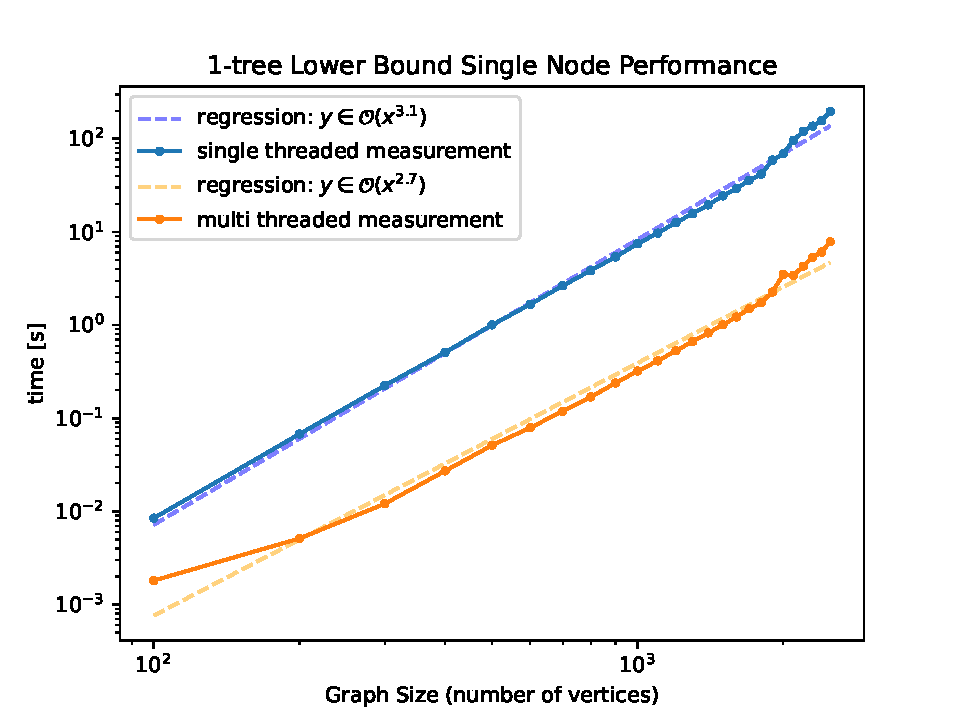
\includegraphics[width=\linewidth,height=0.8\textheight,keepaspectratio]{1-tree-stmt.pdf}
  \end{figure}
  \vfill
\end{frame}

\begin{frame}[t]{1-tree Lower Bound Benchmarking}
  \vfill
  The 1-tree lower bound benefits from parallelization:
  
  \begin{figure}
    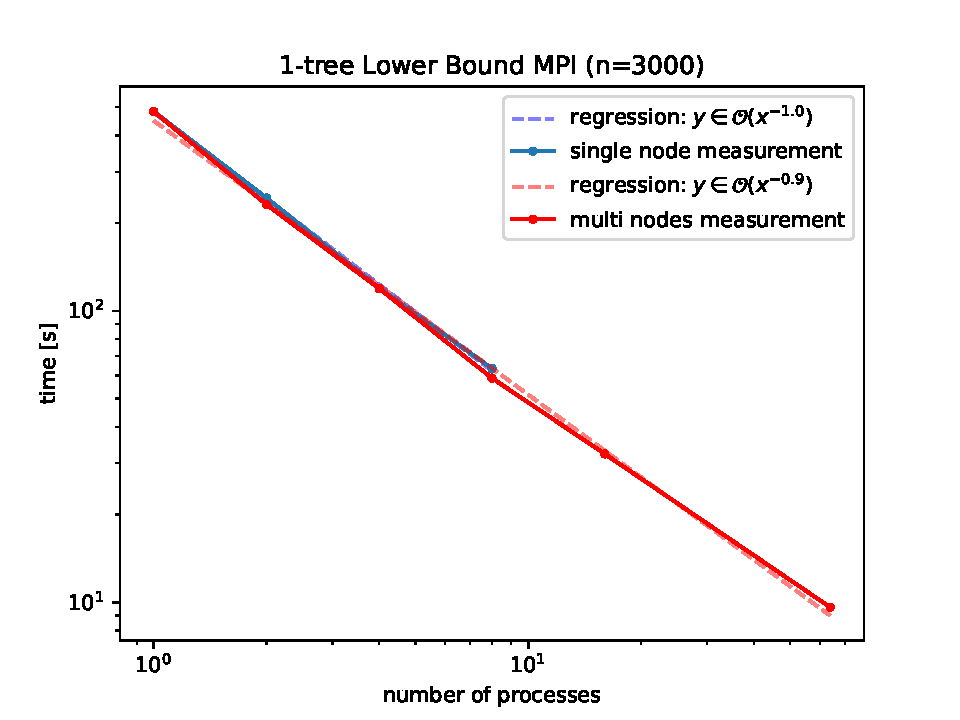
\includegraphics[width=\linewidth,height=0.8\textheight,keepaspectratio]{1-tree-mpi.pdf}
  \end{figure}
  \vfill
\end{frame}
